\documentclass[12pt]{article}
\input{MATH_1060_Preamble.tex}

%\setcounter{page}{1}

\begin{document}
\section*{1.3: Inverse, Exponential, and Logarithmic Functions}

\boxenv{Learning Objectives.}{Upon successful completion of Section 1.3, you will be able to\dots
		
	\begin{itemize}[leftmargin=6mm]
		\item Answer conceptual questions involving inverse, exponential, and logarithmic functions.
		\item Determine the largest possible intervals on which a given function has an inverse.
		\item Find and graph inverse functions.
		\item Use the Change of Base Rule to evaluate logarithms and rewrite exponential \\ expressions.
		\item Evaluate logarithmic expressions.
		\item Solve exponential or logarithmic equations.
	\end{itemize}
	\vspace{-4mm}
}

\vspace{5mm}

\subsection*{Exponential Functions}
\paragraph{Motivation.} Suppose a colony of rabbits doubles in size each month. Let $p_0$ represent the initial population and let $f$ represent a function describing the population after some number of months. We can model this as follows.

\vspace{40mm}

Such a process is modeled by an \textbf{exponential function}.

\vspace{5mm}

\boxenv{Definition.}{An \textbf{exponential function} is a function of the form
\vspace{15mm}
where $a,b\in\R$ and $b>0$. Note that $f(0)=a$. The value of $b$ is referred to as the base.}
		
\vspace{5mm}

\boxenv{Remark.}{Why must we have $b>0$? Suppose $x=\frac{1}{2}$ and $b=-2$. Then\dots
\vspace{15mm}
So, $b>0$ ensures that we avoid complex (non-real) numbers.}

\newpage 

Below are the graphs of \textcolor{blue}{$f(x)=2^x$} and \textcolor{red}{$g(x)=\lp \frac{1}{2} \rp^x$}.

\begin{center}
	\begin{tikzpicture}
    	\begin{axis}[
        	axis x line=middle,
            xmax=4.5, xmin=-6.5,
            axis y line=center,
            ymax=9, ymin=-1,
            xlabel=$x$,ylabel=$y$
		]
                    
        \addplot[name path=f,smooth,domain=-6.5:3,color=blue,samples=100,<->,thick] {2^x};
		\addplot[name path=f,smooth,domain=-3:4.5,color=red,samples=100,<->,thick] {0.5^x};
        \end{axis}
	\end{tikzpicture}
\end{center}

If $b>1$, then $f$ is increasing. If $0<b<1$, then $f$ is decreasing.

\vspace{5mm}

\Example Is the function $h(x)=3\cdot\lp\frac{1}{5}\rp^x$ increasing or decreasing?

\vspace{15mm}

\textbf{Facts about Exponential Functions}
\begin{itemize}
	\item The domain of an exponential function is $\R$, i.e.\ $\lp-\infty,\infty\rp$.
	\item The output of an exponential function is always positive and never zero. Hence, we express the range as $\lp 0,\infty\rp$.
	\begin{itemize}
		\item This means that the equation $b^x=0$ has no solution.
	\end{itemize}
	\item Exponential functions have a horizontal asymptote.
	\item Exponential functions are one-to-one, i.e.\ outputs are never repeated.
	\begin{itemize}
		\item In other words, if $b^x=b^y$, then it must be that $x=y$.
	\end{itemize}
\end{itemize}

\vspace{3mm}

\Example Solve the following exponential equation.
$$2^{3x}=2^{4x-1}$$

\newpage

\textbf{Fractional exponents} represent roots. For instance, $x^{\frac{1}{2}}=\sqrt{x}$. The following relationship can be helpful when working with exponential functions.
$$\sqrt[b]{x^a}=x^{\frac{a}{b}}$$

\Example Rewrite the following expressions in exponent form.

\begin{enumerate}
	\item[\tc{1}] $\sqrt[4]{(2x-3)^3}$
	\vspace{2mm}
	\item[\tc{2}] $\sqrt[8]{12^\frac{3}{8}}$
	\vspace{2mm}
	\item[\tc{3}] $\sqrt[2x]{(1-3x)^4}$
	\vspace{2mm}
\end{enumerate}

\vspace{3mm}

\textbf{The Natural Exponential.} Of particular interest in calculus are exponential functions with the base $e$, i.e.

\vspace{15mm}

where $e\approx 2.71828$. This constant $e$ is an irrational number, meaning that it cannot be expressed as a ratio of integers. We will see the significance of the natural exponential later.

\vspace{5mm}

\textbf{Laws of Exponents.} You should be able to apply some commonly used exponent laws.

\begin{center}
\begin{tabular}{|ccccc|}
	\hline
	& & & & \\
	& $b^xb^y = b^{x+y}$ & & $\disp\frac{b^x}{b^y} = b^{x-y}$ & \\
	& $ $ & & $ $ &  \\
	& $(b^x)^y = b^{xy}$ & & $(ab)^x = a^xb^x$ & \\
	& $ $ & & $ $ &  \\
	& $b^{-x} = \disp\frac{1}{b^x}$ & & $b^{x} = \disp\frac{1}{b^{-x}}$ & \\
	& & & & \\
	\hline
\end{tabular}
\end{center}

\Example Simplify the expression $\sqrt{\sqrt{3}}\sqrt{\sqrt{12}}$.

\newpage

\Example Simplify the expression $\disp\lp\frac{x^{-2}}{x^8}\rp^{-2}$.

\vspace{20mm}

When working with exponents, be careful to avoid a common error.
$$(x-y)^2 \neq x^2-y^2$$

\vspace{5mm}

\subsection*{Inverse Functions}
Very loosely, an inverse function has the effect of ``reversing'' the action of another function.

\vspace{3mm}

\boxenv{Definition.}{An \textbf{inverse function} of a function $f$ is a function $f^{-1}$ such that

\vspace{15mm}

if the inverse exists. Expressed differently, if $y=f(x)$, then $x=f^{-1}(y)$.

\vspace{3mm}

A function $f$ is called \textbf{invertible} if $f^{-1}$ exists.}

\vspace{5mm}

\textbf{Example.} Suppose that $f$ is invertible and $f(2)=3$. Then $f^{-1}(3)=2$.

\vspace{5mm}

\boxenv{Theorem.}{A function $f$ has a unique inverse $f^{-1}$ if and only if $f$ is one-to-one and onto.
\vspace{-4mm}}

\vspace{5mm}

In calculus, we work with functions in such a way that all functions have the property of being \textbf{onto}, so we can generally ignore this condition in this course.

\vspace{3mm}

\textbf{One-to-one} functions pass the horizontal line test. If a function is not one-to-one, we cannot describe an inverse function.

\vspace{3mm}

\begin{center}
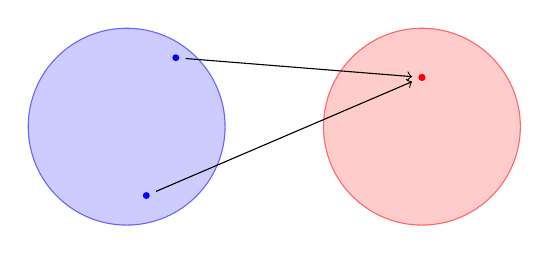
\begin{tikzpicture}[scale=1.25]
    % draw the sets
    \filldraw[fill=blue!20, draw=blue!60] (-1.5,0) circle (1cm);
    \filldraw[fill=red!20, draw=red!60] (1.5,0) circle (1cm);
    % the texts
    %\node at (0,-2) {$f: X \to Y$};

    % the points in the sets (here I just create nodes to use them later on to position
    % the circles and the arrows
    \node (x1) at (-1,0.7) {};
    \node (x2) at (-1.3,-0.7) {};
    \node (y1) at (1.5,0.5) {};
    \node (y2) at (1.5,0.5) {};

    % position the elements in the sets (at the nodes we just created)
    \fill[blue] (x1) circle (1pt);
    \fill[blue] (x2) circle (1pt);
    \fill[red] (y1) circle (1pt);
    \fill[red] (y2) circle (1pt);

    % draw the arrows
    \draw[->] (x1) -- (y1);
    \draw[->] (x2) -- (y2);
\end{tikzpicture}
\end{center}

\vspace{3mm}

\boxenv{Remark.}{The inverse notation is \textbf{not} an exponent.
$$f^{-1}(x)\neq\disp\frac{1}{f(x)}$$
\vspace{-4mm}}

\newpage

\textbf{Finding an Inverse.} Given $y=f(x)$, swap $x$ and $y$, then solve for $y$.

\vspace{2mm}

\Example Find the inverse of the function $f(x)=2x-4$, if it exists.

\vspace{30mm}

\subsection*{Logarithmic Functions}

Exponential functions are one-to-one, so they possess unique inverses. Such inverses are called logarithms.

\vspace{5mm}

\boxenv{Definition.}{A \textbf{logarithmic function} is a function of the form 
\vspace{15mm}
where $a,b\in\R$, $b>0$.}

\vspace{5mm}

\boxenv{Remark.}{The following are equivalent expressions.

\vspace{15mm}

For instance, $2^3=8\,\Longleftrightarrow\log_2 8=3$. This also shows how to solve exponential and logarithmic equations.}

\Example Evaluate the expression $\log_{10}\disp\lp\frac{1}{1000}\rp$.

\vspace{15mm}

\textbf{Working with Logarithms.} The following manipulations are often used when evaluating logarithmic expressions.

\vspace{2mm}

\begin{center}
\begin{tabular}{|ccccc|}
\hline
& & & & \\
& $\log_b b=1$ & & $b^{\log_b x}=x$ & \\
& & & & \\
& $\log_b 1=0$ & & $\log_b b^x=x$ & \\
& & & & \\
\hline
\end{tabular}
\end{center}

\newpage

\Example Solve the following equation using an inverse.
$$2^{x^2+1}=8$$

\vspace{20mm}

\textbf{Finding Inverses Graphically.} If a function is one-to-one, then its inverse may be sketched by reflecting the graph of the function about the line $y=x$.

\begin{center}
            \begin{tikzpicture}
                \begin{axis}[
                	axis x line=middle,
                	xmax=6.5, xmin=-6.5,
                	axis y line=center,
                	ymax=6.5, ymin=-6.5,
                	xlabel=$x$,ylabel=$y$,
                	axis line style={<->}
                    ]
                    \addplot[name path=f,smooth,domain=-6.3:1.8,color=blue,samples=100,<->,thick] {exp(x)};
		    \addplot[name path=g,smooth,domain=0.003:5.9,color=red,samples=100,<->,thick] {ln(x)};	
                    \addplot[name path=h,smooth,domain=-5:5,color=black,dashed,samples=100,<->,thick] {x};
                \end{axis}
            \end{tikzpicture}
        \end{center}
        
\textbf{The Natural Logarithm.} When the base of a logarithm is $e$, then
$$\log_e x=\ln x.$$

This is called the \textbf{natural logarithm.} Note the following properties of natural logarithms.

\begin{center}
\begin{tabular}{|ccc|}
\hline
& & \\
& $\ln e=\log_e e=1$ & \\
& & \\
& $\ln 1=\log_e 1=0$ & \\
& & \\
\hline
\end{tabular}
\end{center}

\boxenv{Remark.}{In the case that no base is written, $\log x=\log_{10} x$.}

\vspace{5mm}

\textbf{Facts about Logarithmic Functions}
\begin{itemize}
	\item The domain of a logarithmic function is $(0,\infty)$. 
	\item The range of a logarithmic function is $(-\infty,\infty)$. 
	\item Logarithmic functions have a vertical asymptote.
	\item Notice that these properties are opposite of exponential functions.
\end{itemize}

\newpage 

\textbf{Laws of Logarithms.} You should be able to apply some commonly used logarithm laws.
\begin{enumerate}
	\item[\tc{1}] $\log_b(xy)=$
	\vspace{4mm}
	\item[\tc{2}] $\log_b\lp x^r\rp=$
	\vspace{2mm}
	\item[\tc{3}] $\log_b\disp\lp\frac{x}{y}\rp=$
	\vspace{2mm}
\end{enumerate}

\Example Solve the following equation using properties of logarithms.
$$\log(x+21)+\frac{1}{2}\log x^2=2$$

\vspace{30mm}

\Example Solve the following equation using properties of logarithms.
$$\ln 10-\ln(7-x)=\ln x$$

\vspace{30mm}


\end{document}